\documentclass[compress,12pt]{beamer}
\usepackage{caption}
\usepackage{subcaption}
\usetheme{Arguelles}
\usepackage{color}
\usepackage{tcolorbox}
\usepackage{xcolor}
\usepackage{booktabs}
\usepackage{algorithm,algpseudocode}
\usepackage{amsfonts, amsmath, amssymb}
\newcommand{\myRed}[1]{\textcolor{red}{#1}}

\title{MATH 512 - Project 3}
\subtitle{}
\event{}
\date{}
\author{Wasif Ahmed, Haoxiang Deng, Jacob Fein-Ashley, Kanav Malhotra, Longzhe Yang}


\begin{document}

\frame[plain]{\titlepage}

\section{Question 1}



\begin{frame}{Question 1 Overview}
      \begin{itemize}
            \item Let $W_t$ be a standard Wiener process, with drift parameter zero and variance parameter $\sigma^2 = 1$.
            \item We divide the interval $[0,2]$ into $L$ subintervals $[t_i, t_{i+1}]$, where $t_i = i\delta t$ and $\delta t = 2/L$.
            \item Let $W_i = W(t_i)$ and $\delta W_i = W_{i+1} - W_i$.
            \item We verify numerically that:
            \begin{itemize}
                  \item $\sum_{i=0}^{L-1} |\delta W_i|$ is unbounded as $\delta t$ goes to zero.
                  \item $\sum_{i=0}^{L-1} \delta W_i^2$ converges to 2 in probability as $\delta t$ goes to zero.
            \end{itemize}
      \end{itemize}
      
\end{frame}

\begin{frame}{Question 1 Response}
      Refer to Figure~\ref{fig:convergence1}

      \begin{figure}[H]
      \centering
      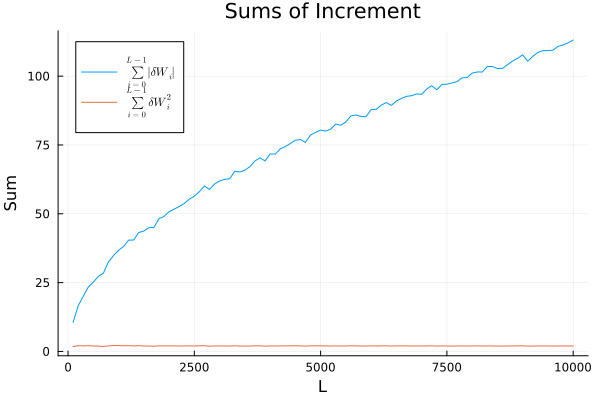
\includegraphics[scale=0.32]{imgs/convergence1.png}
      \caption{Stochastic Plots}
      \label{fig:convergence1}
      \end{figure}

Notice that as the $L$ parameter increases, the $|\delta W_i|$ term is unbounded while $\delta W_i^2$ converges to $2$ in probability.
\end{frame}
\section{Question 2}
\begin{frame}{Question 2a}

      \begin{figure}[H]
            \centering
            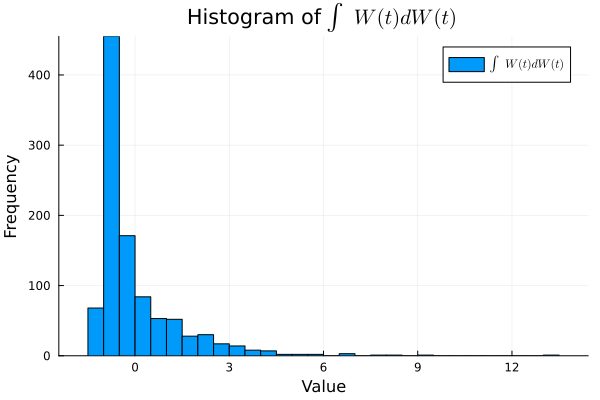
\includegraphics[scale=0.5]{imgs/2a.png}
            \caption{2a}
            \label{fig:2a}
      \end{figure}

\end{frame}

\begin{frame}{Question 2b}

      \begin{figure}[H]
            \centering
            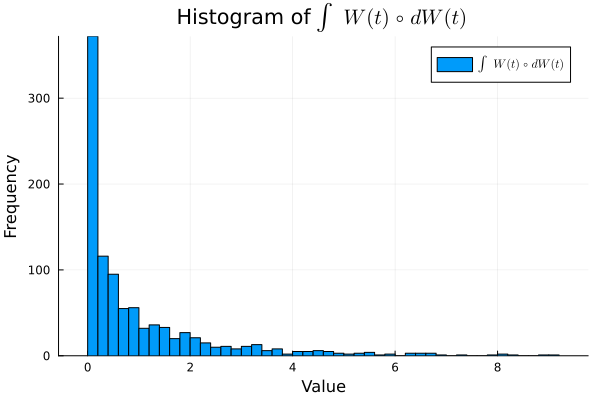
\includegraphics[scale=0.5]{imgs/2b.png}
            \caption{2b}
            \label{fig:2b}
      \end{figure}
\end{frame}

\begin{frame}{Question 2c}

      \begin{figure}[H]
            \centering
            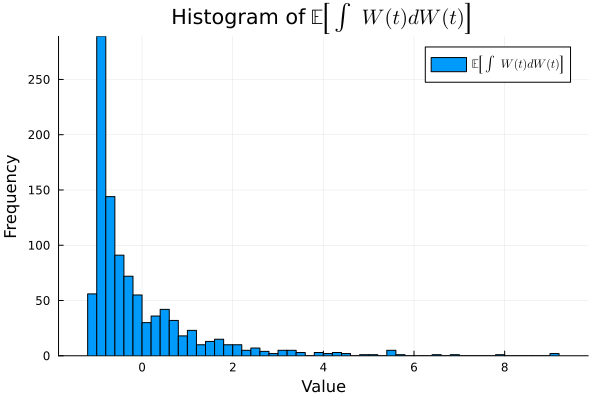
\includegraphics[scale=0.5]{imgs/2c.png}
            \caption{2c}
            \label{fig:2c}
      \end{figure}
\end{frame}


\begin{frame}{Question 2d}
      \begin{figure}[H]
            \centering
            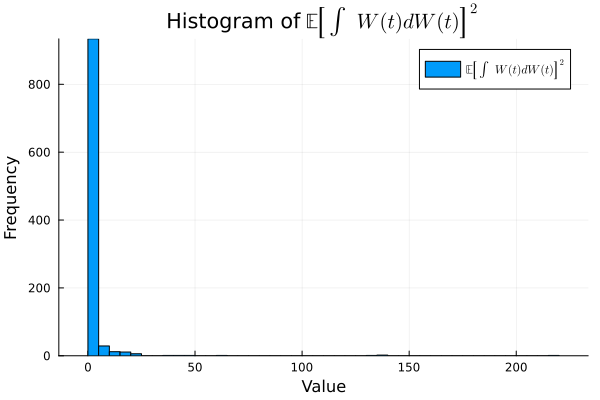
\includegraphics[scale=0.5]{imgs/2d.png}
            \caption{2d}
            \label{fig:2d}
      \end{figure}
\end{frame}


\begin{frame}{Question 2e}
      \begin{figure}[H]
            \centering
            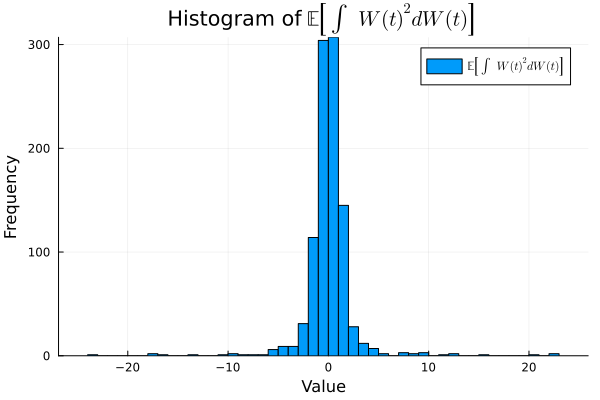
\includegraphics[scale=0.5]{imgs/2e.png}
            \caption{2e}
            \label{fig:2e}
      \end{figure}

\end{frame}

\begin{frame}{Question 2f}
      \begin{figure}[H]
            \centering
            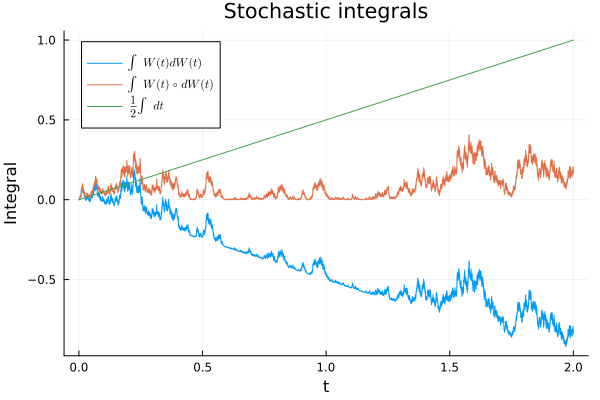
\includegraphics[scale=0.5]{imgs/2f.png}
            \caption{2f}
            \label{fig:2f}
      \end{figure}

\end{frame}

\section{Question 3}
\begin{frame}{Question 3}
\end{frame}


\section{Question 4}
\begin{frame}{Question 4}
\end{frame}

\section{Question 5}
\begin{frame}{Question 5}
Algorithm for computing the mean exit time function $\tau(x)$ for $x \in [0.5, 3]$:
\begin{algorithmic}
      \For{$i = 1$ to $1000$}
            \State $dw \gets \sqrt{dt} \times \text{randn}()$
            \State $x \gets x_0$
            \For{$j = 1$ to $n$}
                  \State $x \gets \text{euler\_maruyama}(x, dt, dw)$
                  \State $dw \gets \sqrt{dt} \times \text{randn}()$
                  \If{$x < a$ or $x > b$}
                        \State $\text{exit\_times}[i] \gets j \times dt$
                        \State \textbf{break}
                  \EndIf
            \EndFor
      \EndFor
\end{algorithmic}
\end{frame}

\begin{frame}{Question 5 Continued}
\begin{figure}[H]
            \centering
            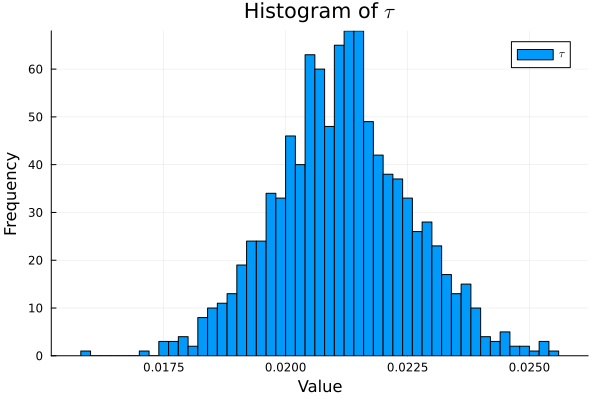
\includegraphics[scale=0.5]{imgs/5.png}
            \caption{2e}
            \label{fig:2e}
      \end{figure}

\end{frame}

\End
\begin{frame}[plain,standout]
      \centering
      Questions?
\end{frame}

\end{document}